\documentclass[justified]{tufte-handout}
\usepackage{../braph2_tut}
%\geometry{showframe} % display margins for debugging page layout

\title{Pipeline for Comparison of Weighted Structural Data between Groups of Subjects}

\begin{document}

\maketitle

\begin{abstract}
\noindent
In this tutorial, we will upload a file containing the pipeline with the different steps to compare two groups of subjects using \emph{structural data} (check tutorial \emph{Group of Subjects with Structural Data}) and weighted undirected graphs. This Tutorial explains how to perform group analyses and comparisons with this kind of data.
\end{abstract}

\tableofcontents

\fig{figure*}
	{fig:01}
	{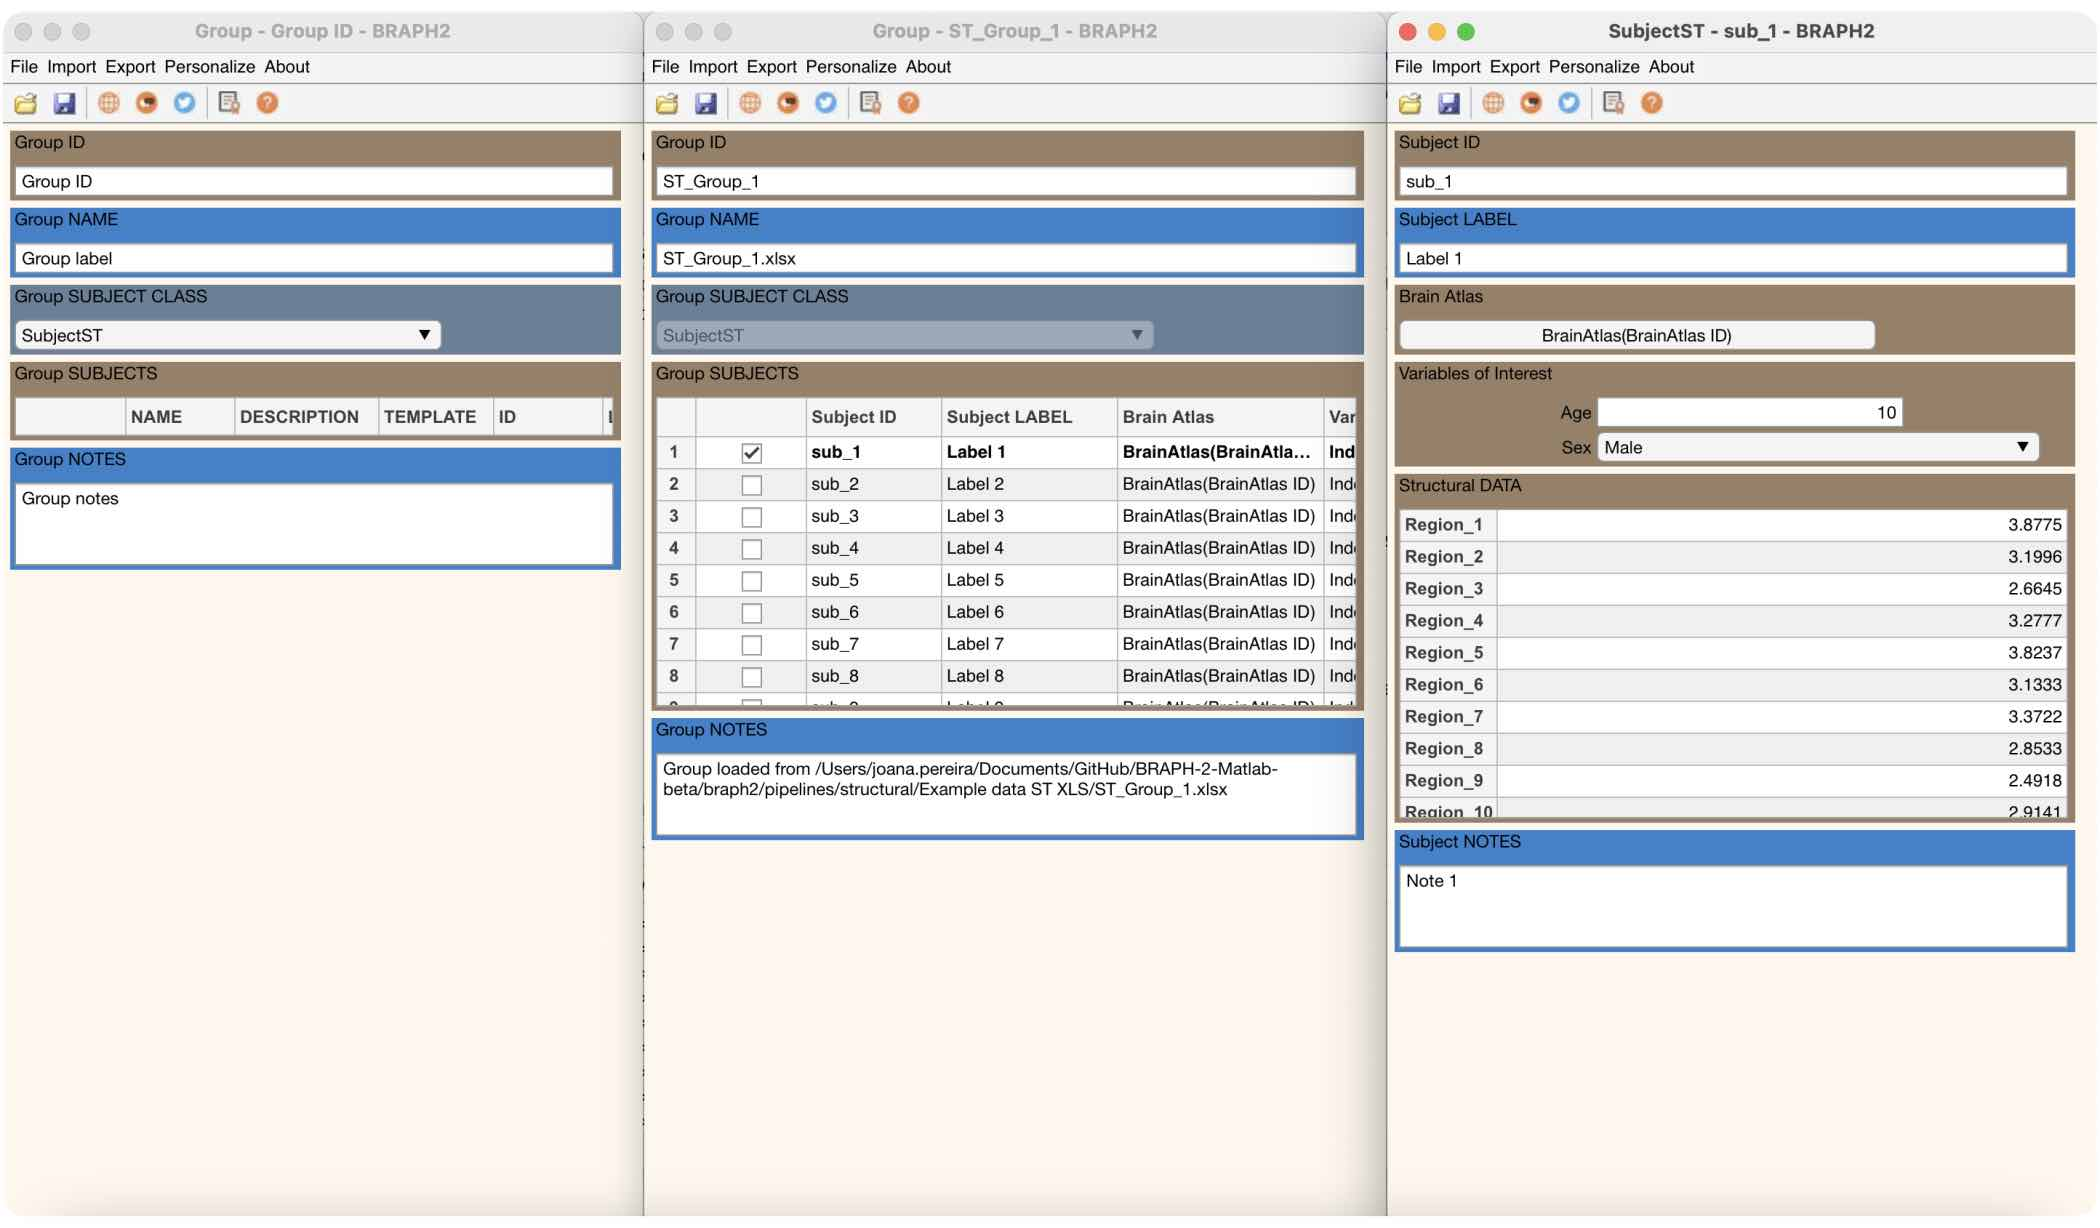
\includegraphics{fig01.jpg}}
	{GUI for working with the pipeline to compare two groups of subjects with \emph{structural data} using a weighted undirected analysis (Figure TBD)}
	{
	Full graphical user interface to perform group comparisons with \emph{structural data} in BRAPH~2.0. 
	}

\clearpage
\section{Open the GUI}

The pipeline GUI can be opened by typing \code{braph2} in MatLab's terminal, which allows you to select a pipeline, in this case, \fn{pipeline\_structural\_comparison\_wu.braph2} (containing the steps required to perform your analysis).

To open the GUI and upload the structural comparison pipeline, you can also do it from the command line by typing the commands in \Coderef{cd:launch}.
%
\begin{lstlisting}[
	label=cd:launch,
	caption={
		{\bf Code to launch the GUI to upload a pipeline file to compare two groups of subjects.}
		This code can be used in the MatLab command line to launch the GUI to upload a pipeline file.
	}
]
pip = Pipeline(); ¥\circled{1}\circlednote{1}{creates a new object \code{Pipeline} to upload the steps to perform an analysis or comparison.}¥

gui = GUIElement('PE', pip); ¥\circled{2}\circlednote{2}{creates a GUI to upload the files into the pipeline.}¥
gui.get('DRAW')¥\circled{3}\circlednote{3}{draws the GUI.}¥
gui.get('SHOW') ¥\circled{4}\circlednote{4}{shows the GUI.}¥
\end{lstlisting}

Once the pipeline is uploaded, you can see a GUI that contains different steps: to upload a brain atlas, to upload the structural data of two groups, analyze them, and finally, to compare the groups (\Figref{fig:02}a). 

\section{Step 1: Load the Brain Atlas}
\Figref{fig:02} shows how to upload and plot the brain atlas that you used to extract the \emph{structural data} for your analysis. For more information on where to find different atlases or how to change plotting settings on the brain surface, check the \emph{Brain Atlas} tutorial.

\fig{figure*}
	{fig:02}
	{
	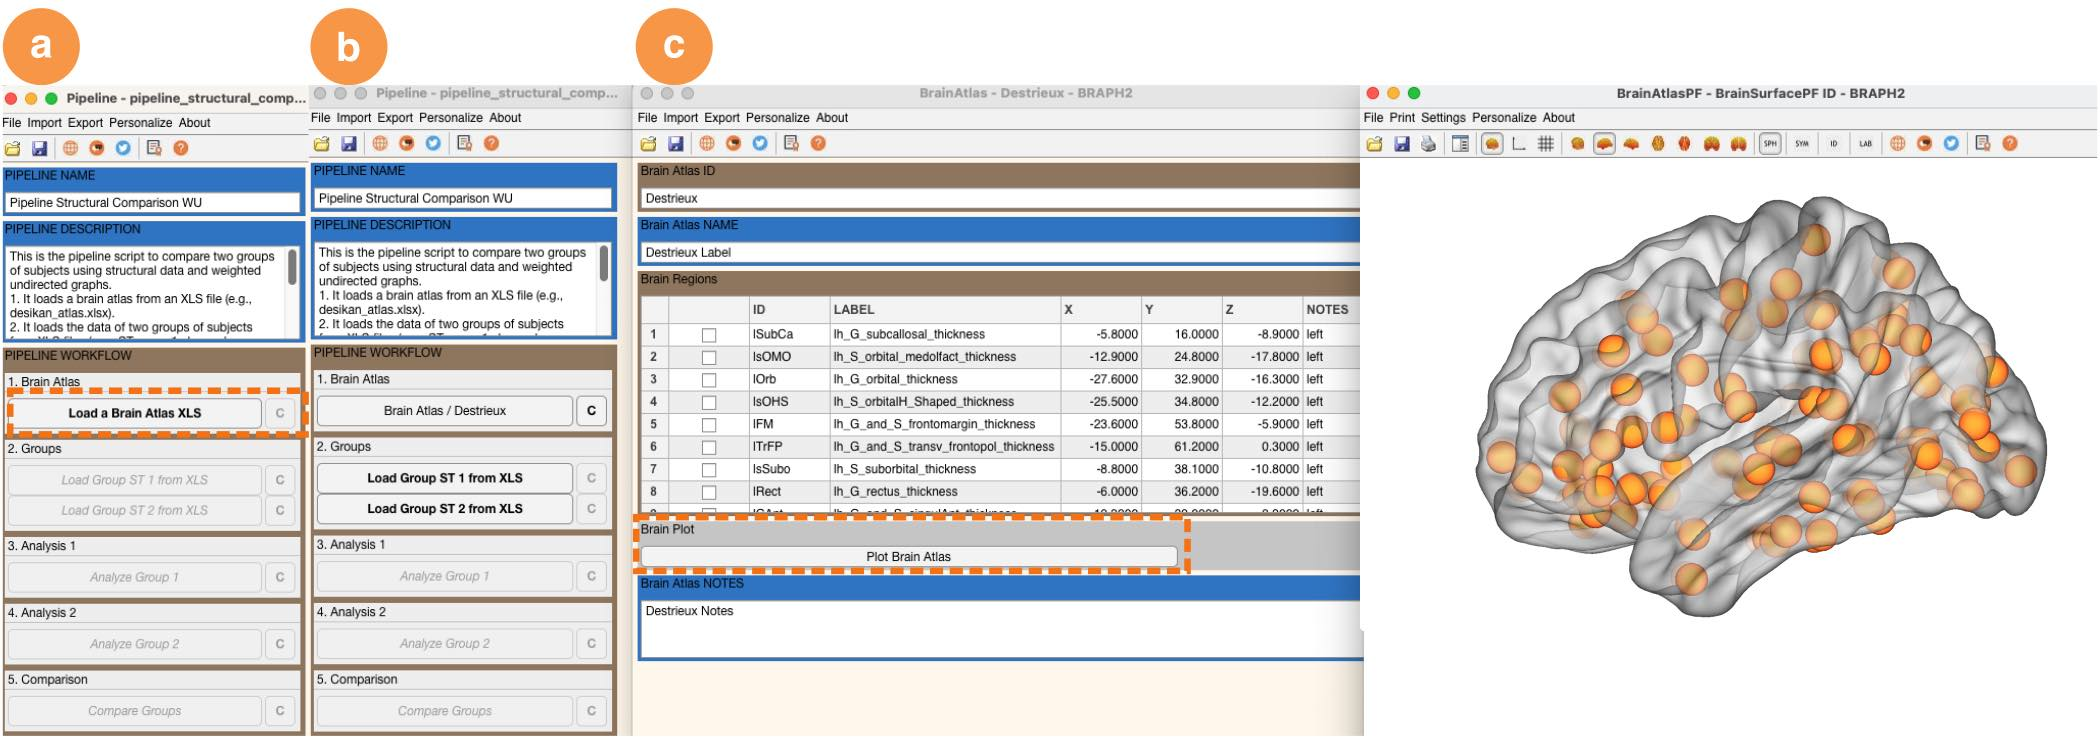
\includegraphics{fig02.jpg}
	}
	{Uploading the Brain Atlas}
	{
	Steps to upload the brain atlas:
	{\bf a} Click on \fn{Load Atlas} from the pipeline GUI.
	{\bf b} Navigate to the BRAPH~2.0 folder \fn{atlases} and select one of the atlas files, in this example the \fn{destrieux\_atlas.xlsx}. {\bf c} You can also plot the brain atlas by pressing \fn{Plot Brain Atlas}. 
	}
 
\section{Step 2: Load the Structural Group Data}

After you loaded the brain atlas, you can upload the \emph{structural data} for each group as shown in \Figref{fig:03}. A new interface will be shown containing the data for the group you just selected. You can open each subject’s structural values by selecting
the subject, right click, and select “Open selection” (for more information check tutorial \emph{Group of Subjects with Structural Data}).
	
	\fig{figure}
	{fig:03}
	{
	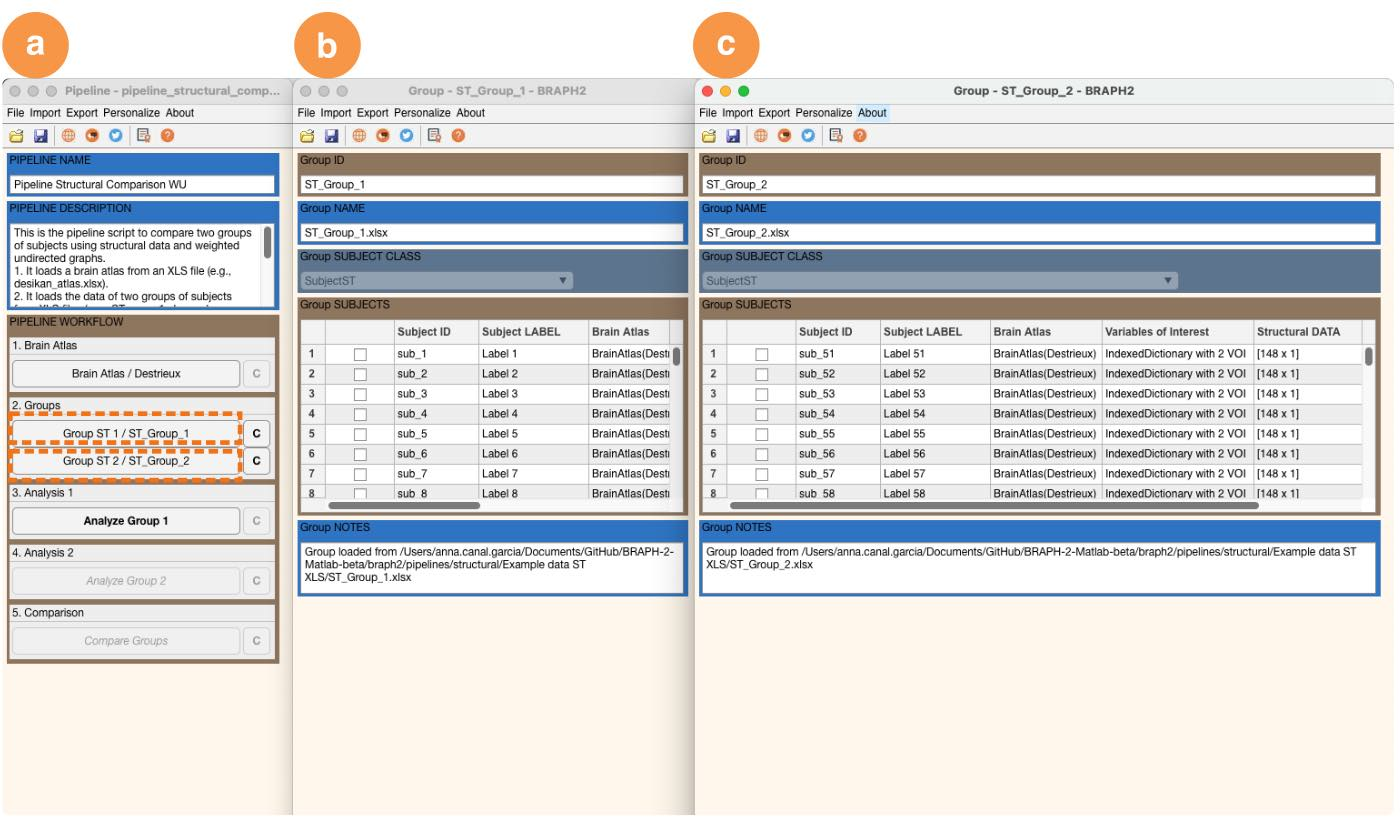
\includegraphics{fig03_medium.jpg}
	}
	{Loading the Groups Data}
	{
	{\bf a} From the pipeline GUI, click on \fn{Load Group ST 1 XLS} to load the data of group 1, and \fn{Load Group ST 2 XLS} to load the data of group 2.
	{\bf b} Data for group 1 is uploaded. {\bf c} Data for group 2 is uploaded.
	}

\section{Step 3: Analysing the Data of Group 1}
 
After you have loaded the data, you can analyze the data of your first group by clicking on \fn{Analyze Group 1} (\Figref{fig:04}a). A new interface will be shown that allows you to pre-calculate network measures for each group and explore them (\Figref{fig:04}b-c). First of all, you can specify the parameters for constructing the graph from the structural group data: you can select the statistical test to calculate correlations in structural values between pairs of brain regions (\Figref{fig:04}d), and you can decide how you want to analyze the negative weights from the correlation. 

Importantly, the parameters you select for this analysis (graph and measures parameters) will be fixed for the analysis of the second group and for the group comparisons.

	\fig{figure}
	{fig:04}
	{
	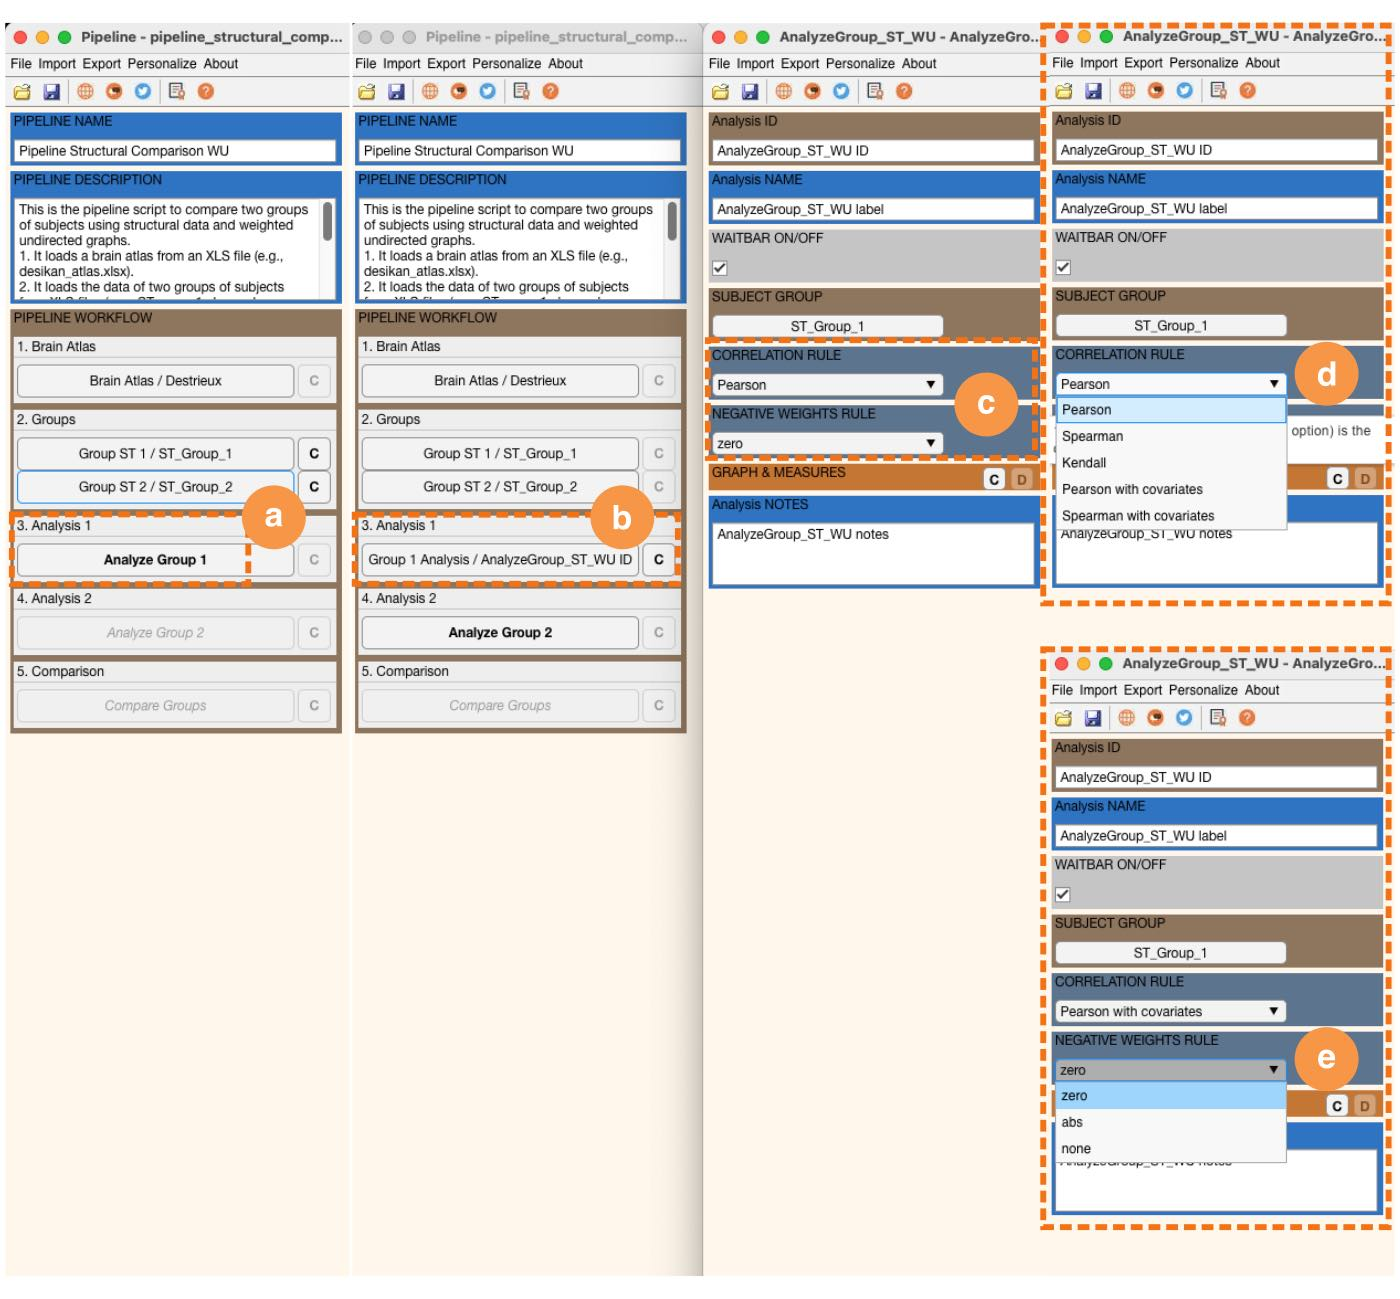
\includegraphics{fig04.jpg}
	}
	{Analyze the Group Data}
	{
	{\bf a} Click on \fn{Analyze Group 1} in the pipeline's GUI.
        {\bf b} After clicking on \fn{Analyze Group 1} in the pipeline's GUI, a new window will appear where first you can select the parameters for the graph construction {\bf c}. In this pipeline, you can select the statistical test to be used for the correlations {\bf d}, and what you want to do with the negative correlation weights {\bf e}.
	}

	\fig{figure}
	{fig:05}
	{
	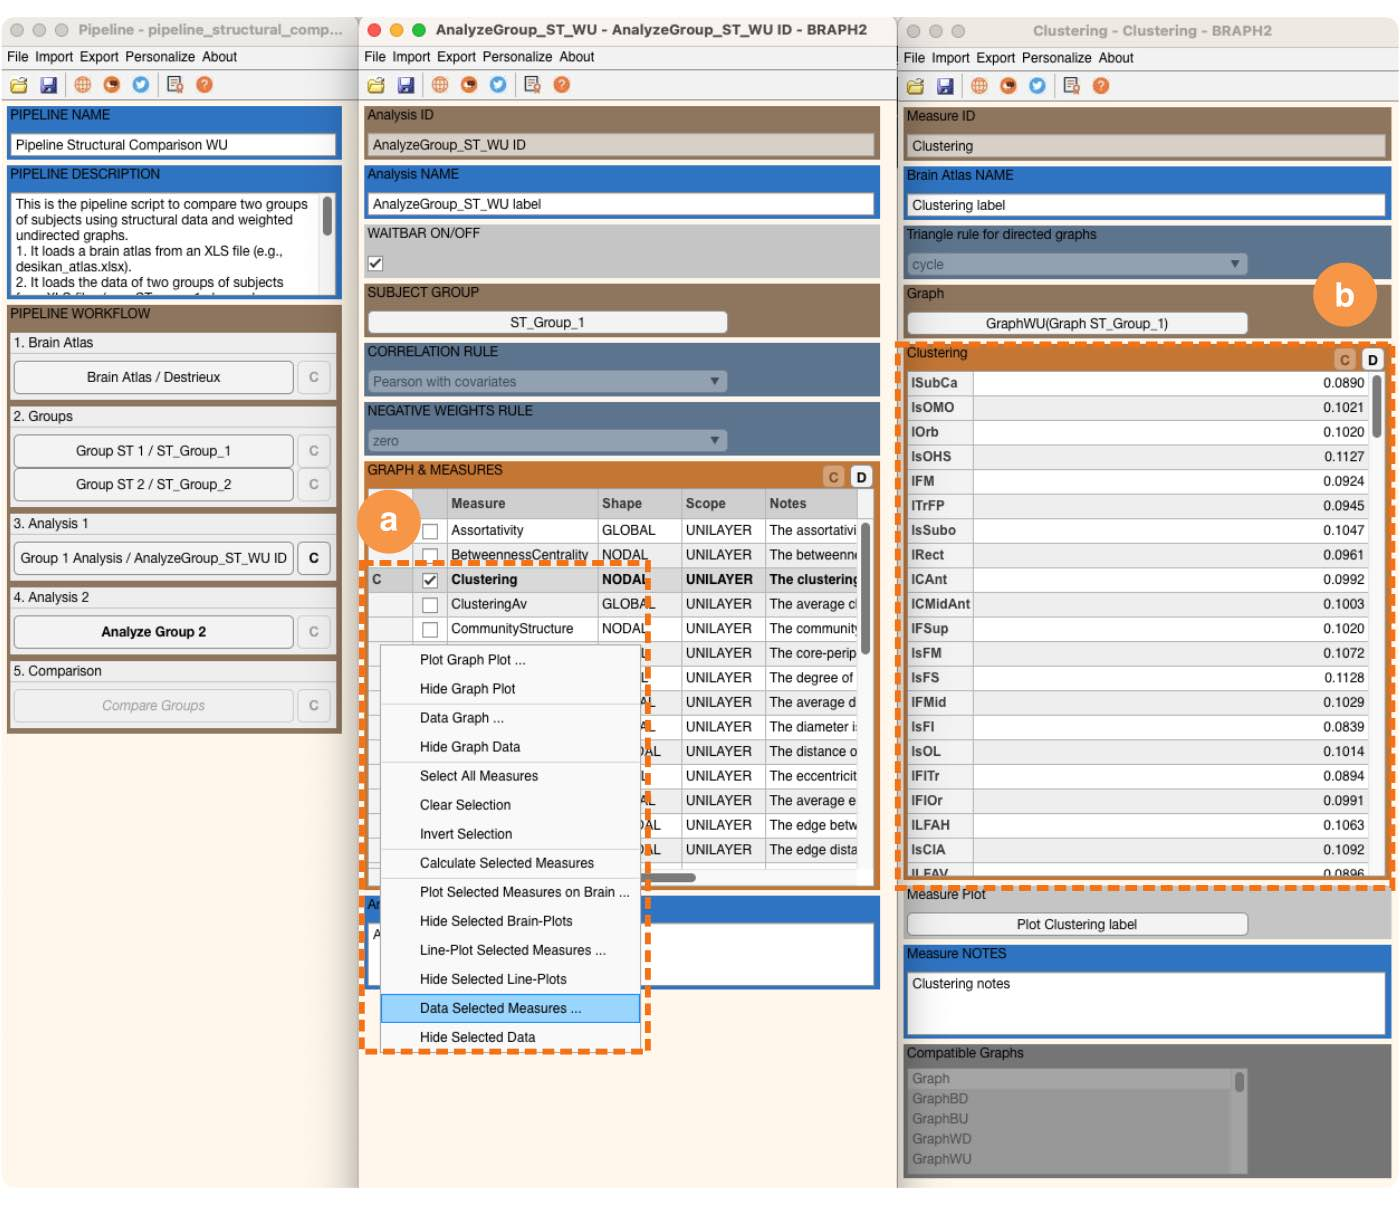
\includegraphics{fig05.jpg}
	}
	{Check and set the rules and/or parameters of a measure before its calculation}
	{
	{\bf a} Click on \fn{Data Selected Measures} after selecting the measure.
	{\bf b} This new window shows the array of values for the measure, in this case \fn{Clustering}.
 	{\bf c} This new window shows the array of values for the measure, in this case \fn{Clustering}.
  	{\bf d} After the calculation of the measure, a new table appears with the measure results, and the rule is blocked (in blue).
	}
 
 After setting these parameters, you can calculate some graph measures (\Figref{fig:05}). First of all, you need to ensure the measure is using the rule or parameter that you wish (not all measures have rules or parameters). As an example, we can select the measure \fn{Clustering} and right-click on the top of the table (\Figref{fig:05}a), in the \fn{GRAPH $\&$ MEASURES} panel, and press “Data Selected Measures”. 
 Next, the measure window will appear, allowing you to choose the rules or parameters (\Figref{fig:05}b). In this instance, the rule applies to the calculation of triangles in directed graphs. However, since we're working with an undirected graph, we will keep the default option (\Figref{fig:05}b).
After the rule is set, you can calculate the measure by pressing the "C" (\Figref{fig:05}c) and the results will appear in a new table within the same panel (\Figref{fig:05}d). Also notice that after the measure is calculated, the rule is blocked (\Figref{fig:05}d).
 
 If you want to visualize the results, select the measure and press \fn{Plot Selected Measures on Brain} in the analysis' GUI (\Figref{fig:06}a). In settings ((\Figref{fig:06}b), you can change the visualization of the plots and save them. 
 
	\fig{figure}
	{fig:06}
	{
	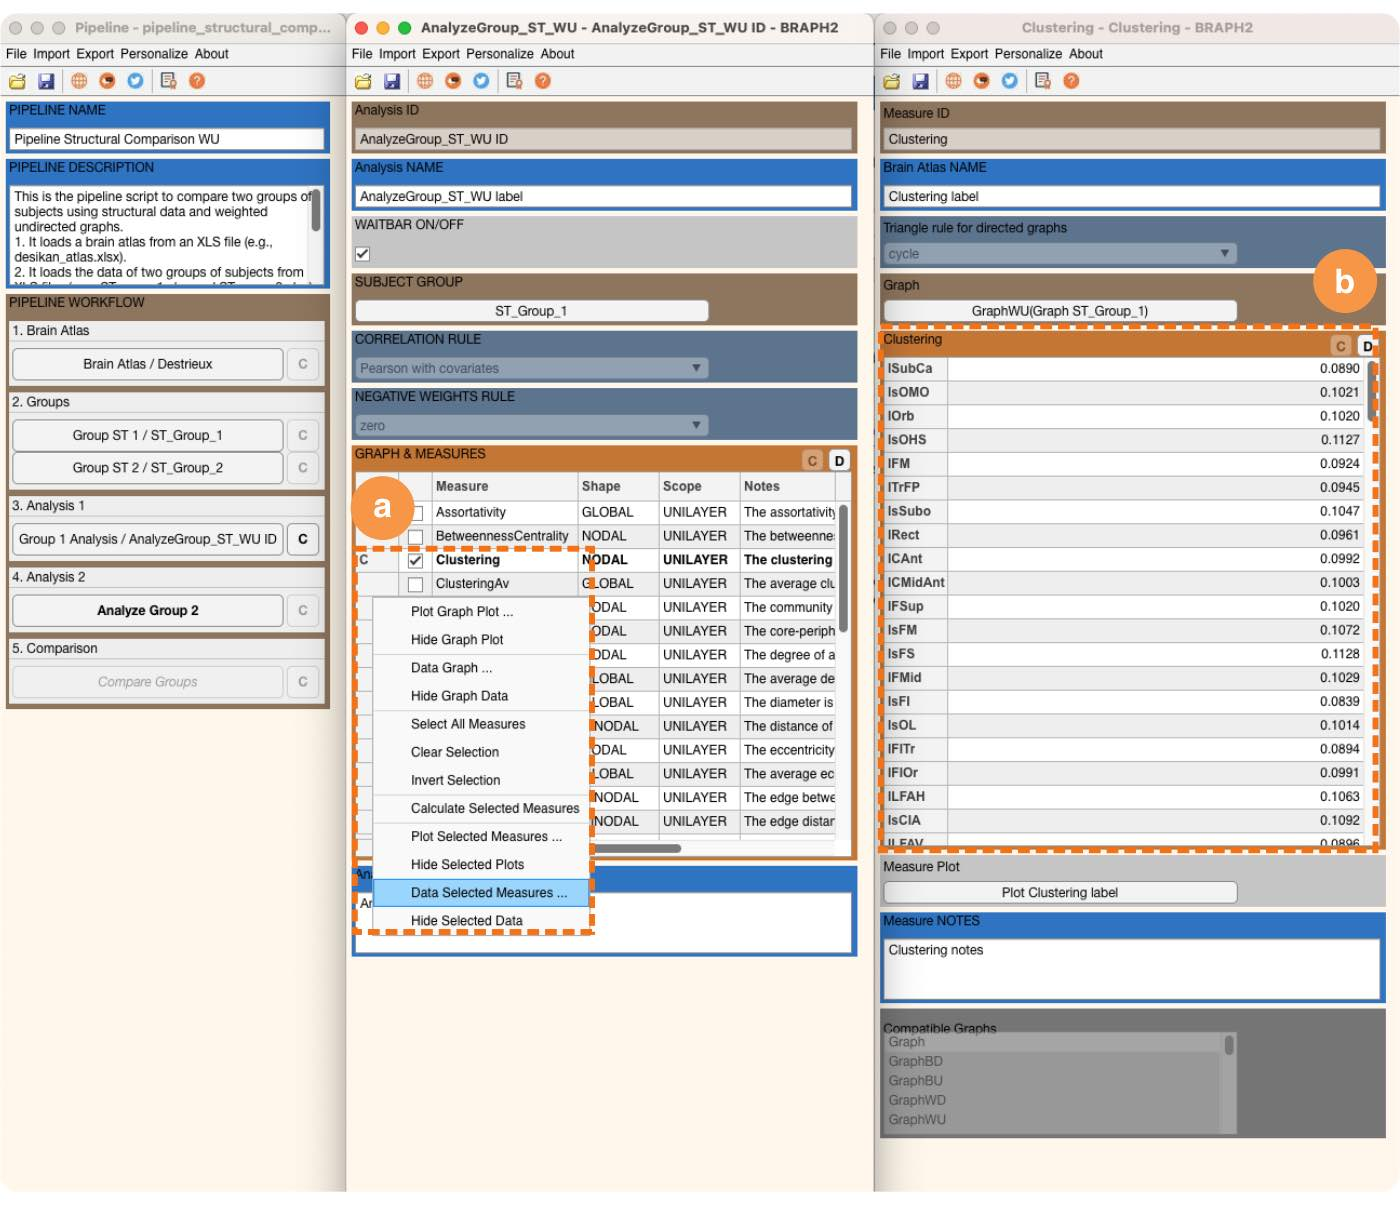
\includegraphics{fig06.jpg}
	}
	{Visualize a connectivity measure in a brain plot (Figure TBD)}
	{
	{\bf a} Click on \fn{Plot Selected Measures on Brain} in the analysis' GUI.
        {\bf b} In the new window, press the button settings to obtain further visualization options of the results.
        {\bf c} Press on Measures to show the values of \fn{Clustering}. The size of the spheres and the color are proportional to the measure's value.   
	}
 
 Finally, when you do right click, in the \fn{GRAPH $\&$ MEASURES} panel, there are other options you can explore such as \fn{Plot Graph Plot} (connectivity adjacency matrix) as well as Data Graph (labels of brain regions, values of the adjacency matrix, options to plot matrix and histogram), all of which can also be saved.
  
\section{Step 4: Analysing the Data of Group 2}

After the analysis of group 1, you can proceed with the analysis of the second group by clicking on \fn{Analyze Group 2}. You will notice that, in the new window that is shown, the parameters you selected for group 1 are already selected and fixed for this analysis (both graph and measure parameters). If you realize that some of the options you previously selected are not the ones you would like, you can reset the analysis parameters of group 1 by clicking on the C checkbox next to it.

	\fig{figure}
	{fig:07}
	{
	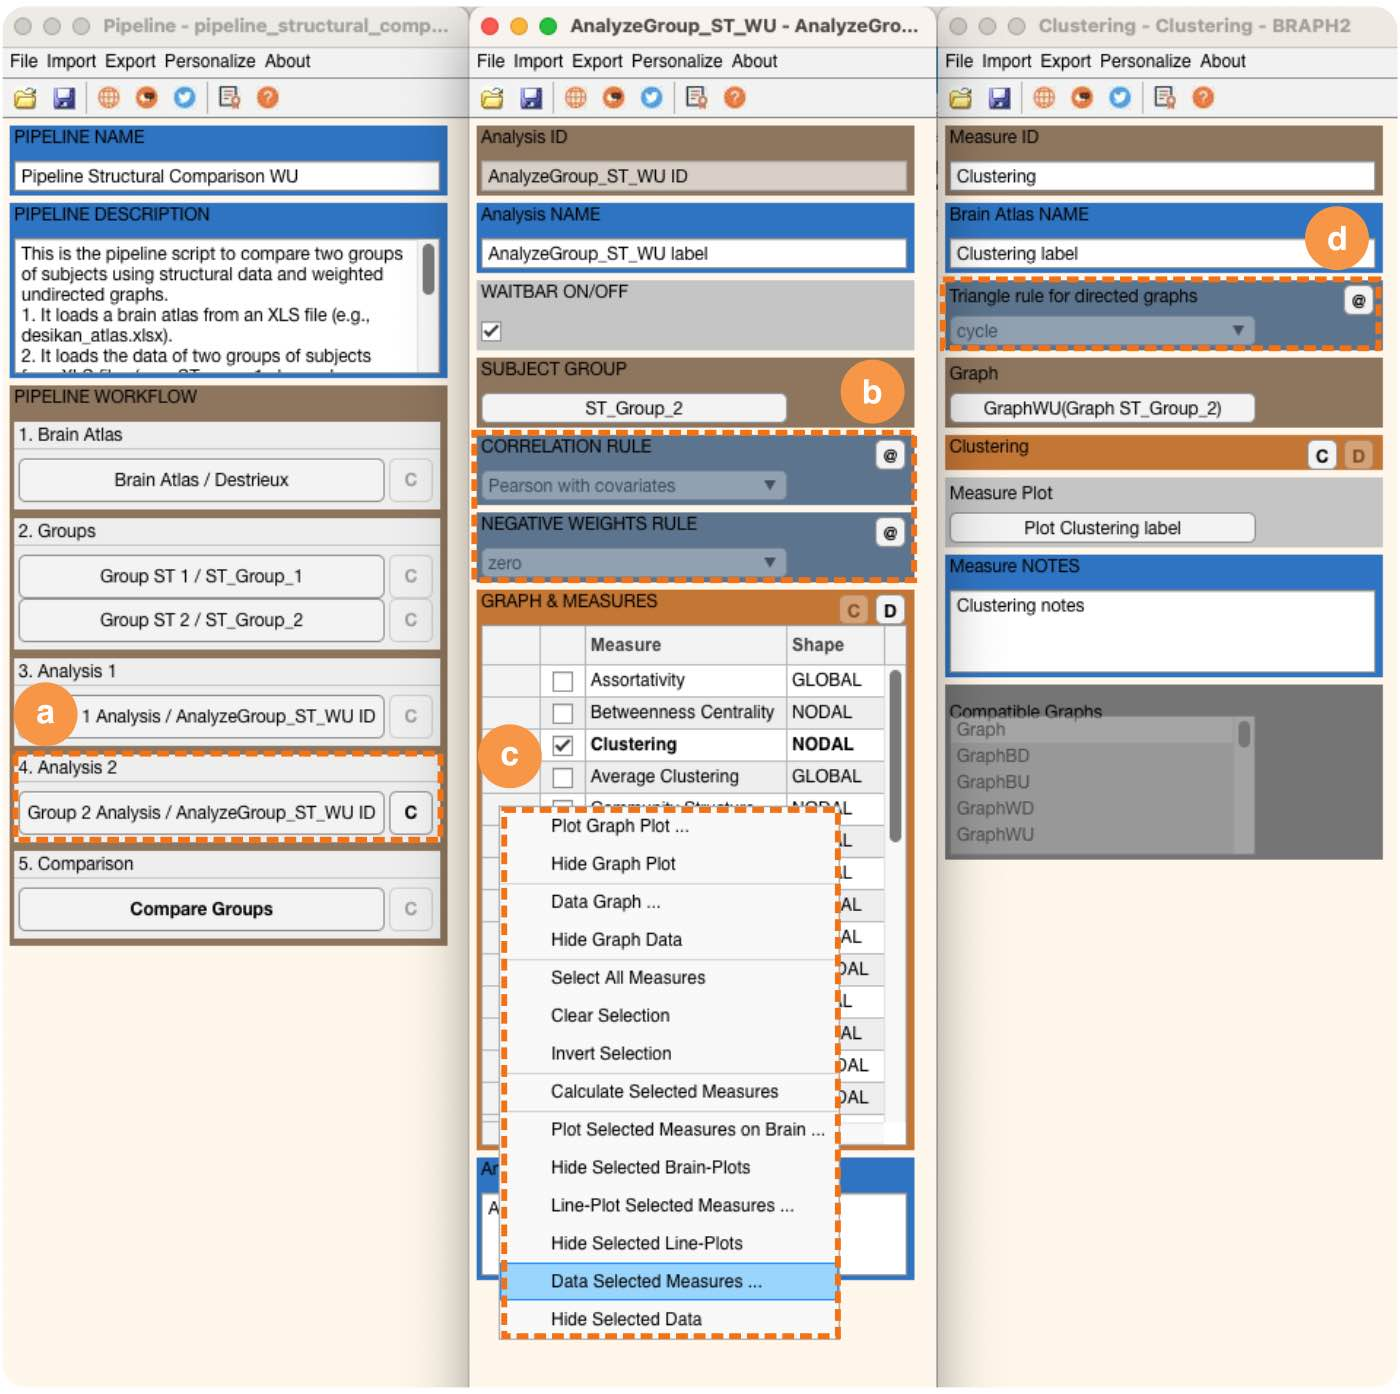
\includegraphics{fig07.jpg}
	}
	{Parameters blocked in Analysis of Group 2}
	{
	{\bf a} Click on \fn{Analysis 2} in the pipeline's GUI.
	{\bf b} In this new window, you can see that the graph properties such as \fn{Correlation rule} and \fn{Negative weights rule} are blocked since they are the same as the ones set in the analysis of group 1. If you select a measure, in this case \fn{Clustering}, and press \fn{Data Selected Measures} {\bf c}, you can observe that the measure's rules and parameters are also set in case you calculated the measures in analysis 1, and if not, you can set the rule by pressing at the "@" {\bf d}.
	}
 
\section{Step 5: Comparing Groups}

Once you have explored the network measures for each group, you can proceed with their statistical comparison. To do this, you should click on \fn{Compare Groups} (\Figref{fig:08}a) and in the new window select if you want a waiting bar and verbose functions ON while you wait for the analysis to finish, as well as how many permutations you want to use to assess differences between groups {\Figref{fig:08}b} and, if the groups are not independent but represent the same subjects in two different points in time, you can select the longitudinal comparison option, which will permute the values within each subject {\Figref{fig:08}b}. We set the permutations to 10 for computational time purposes {\Figref{fig:08}c}, but for your research analysis we recommend using 1000 or 10000 permutations. Finally, you can select the graph measures you want to compare between groups and once you have selected all the measures you are interested in, you should right click and select \fn{Calculate all selected comparisons} {\Figref{fig:08}d}. If you turn ON the wait bar and verbose functions, two window bars will open that show you at which point in time the analysis is. There is one last option on this GUI that you can select to save intermediate results during the permutations.

	\fig{figure}
	{fig:08}
	{
	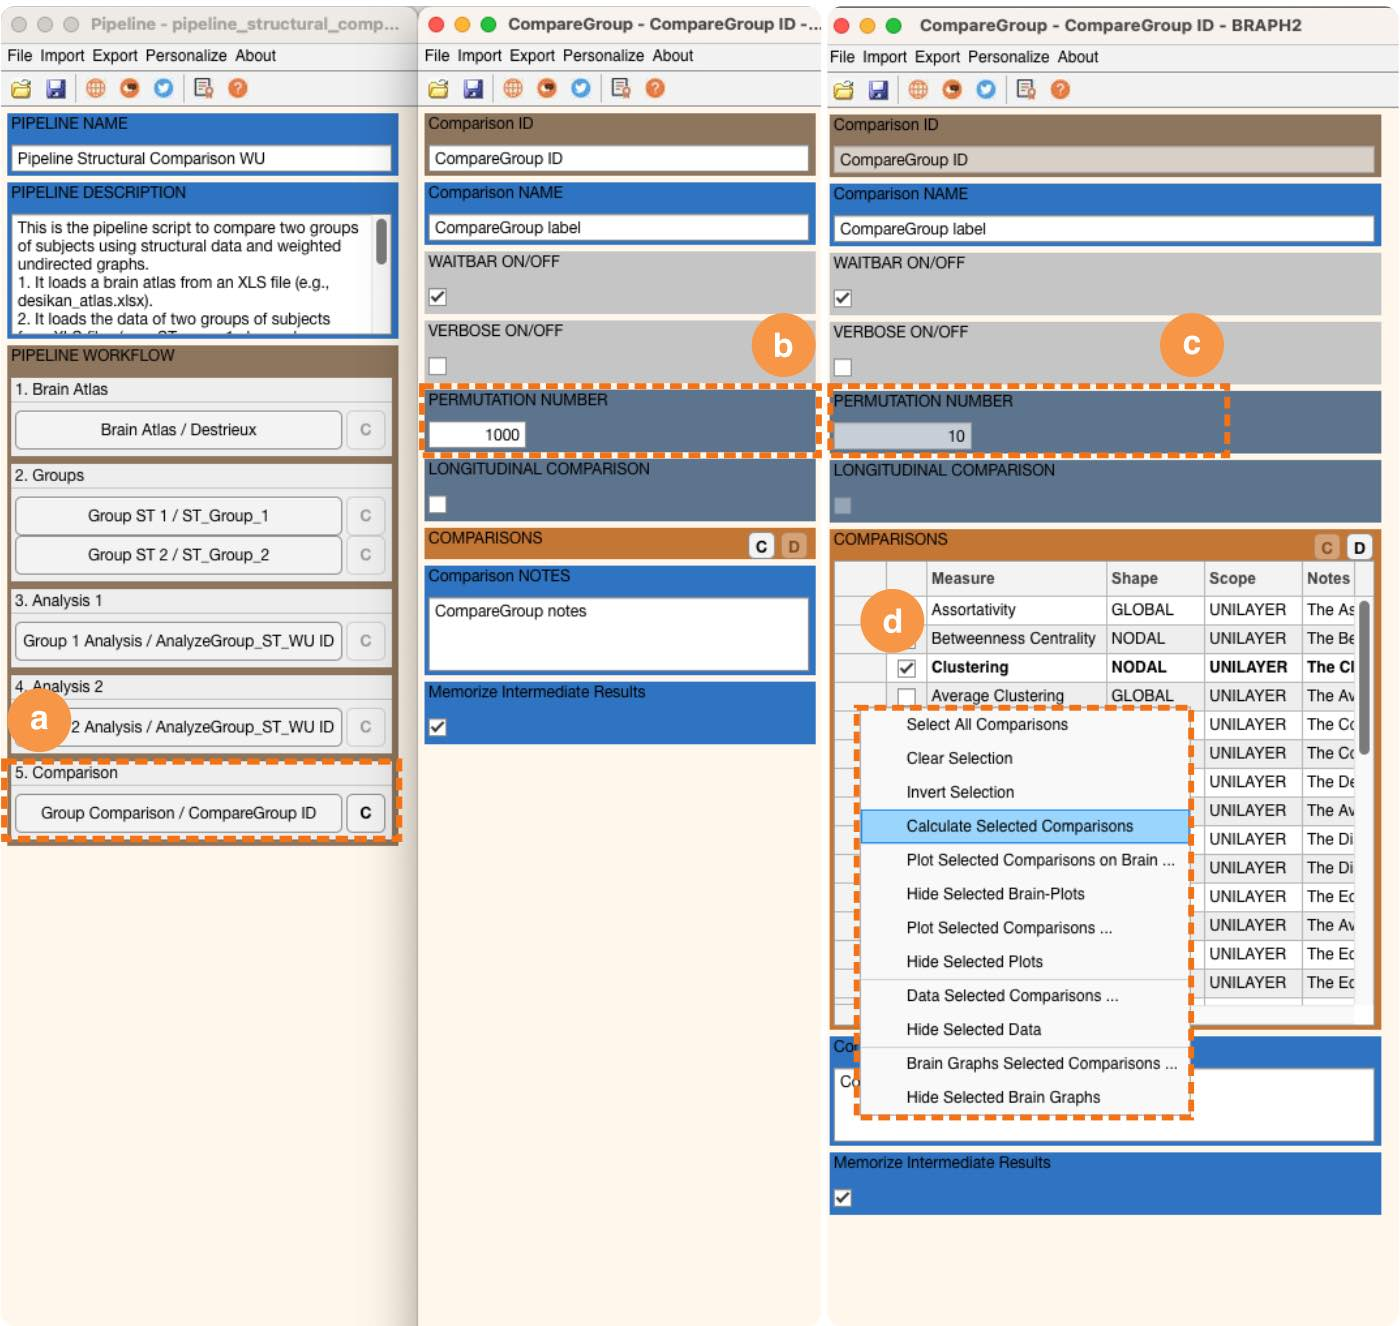
\includegraphics{fig08.jpg}
	}
	{Compare the Group Data}
	{
	{\bf a} Click on \fn{Compare Groups} in the pipeline's GUI.
	{\bf b} In this new window, you can select what to turn ON/OFF the wait bar and verbose functions, you can change the number of permutations, and whether to perform a longitudinal group comparison. We set the number of permutations to 10 for this tutorial {\bf c}. Finally, you can calculate the comparison of some graph measures between groups {\bf d}.
	}

 	\fig{figure}
	{fig:09}
	{
	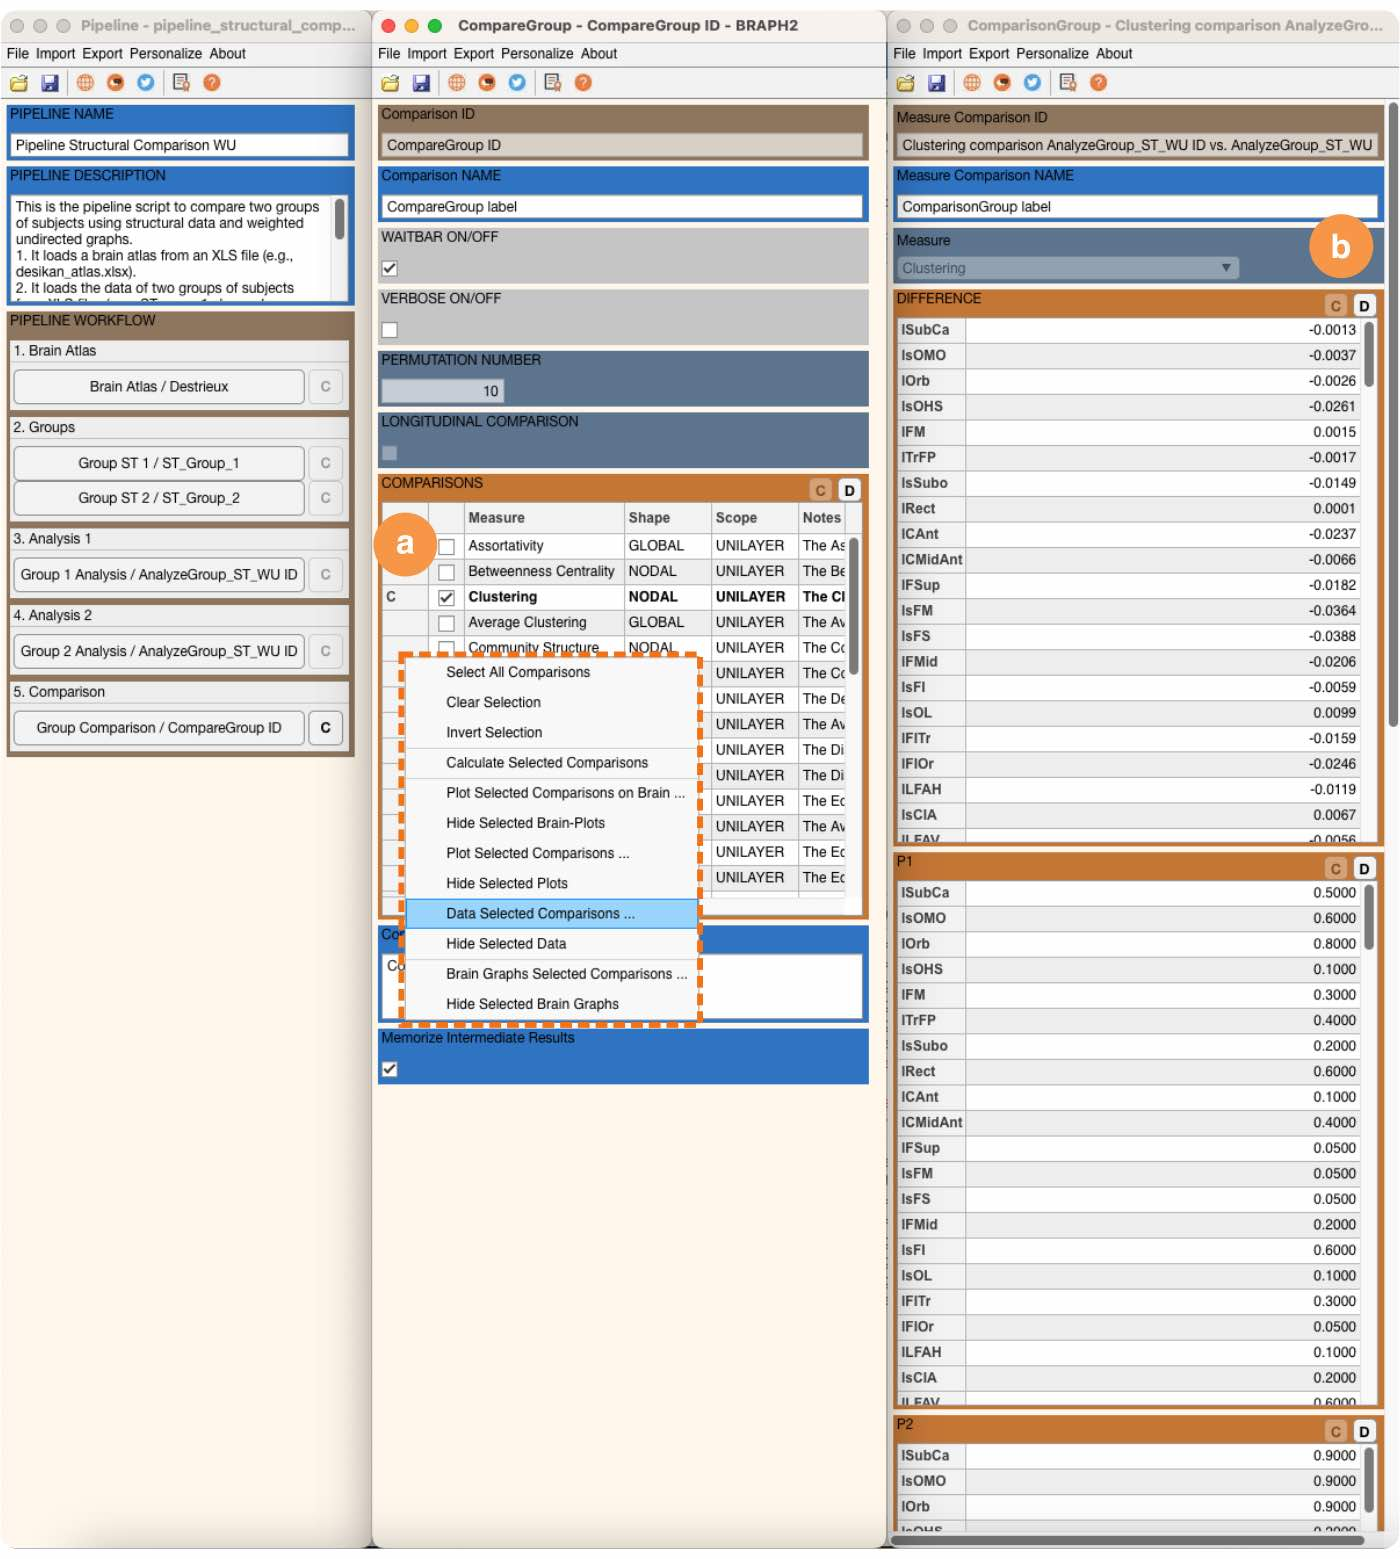
\includegraphics{fig09.jpg}
	}
	{Visualize the comparison results in a table}
	{
	{\bf a} Click on \fn{Data Selected Comparisons} in the Comparisons panel.
	{\bf b} In this new window, you can see the results from the comparison: the difference values between groups, the p-values (1-tailed and 2-tailed), as well as the confidence intervals.
	}
\end{document}